% Options for packages loaded elsewhere
\PassOptionsToPackage{unicode}{hyperref}
\PassOptionsToPackage{hyphens}{url}
%
\documentclass[
]{article}
\usepackage{amsmath,amssymb}
\usepackage{iftex}
\ifPDFTeX
  \usepackage[T1]{fontenc}
  \usepackage[utf8]{inputenc}
  \usepackage{textcomp} % provide euro and other symbols
\else % if luatex or xetex
  \usepackage{unicode-math} % this also loads fontspec
  \defaultfontfeatures{Scale=MatchLowercase}
  \defaultfontfeatures[\rmfamily]{Ligatures=TeX,Scale=1}
\fi
\usepackage{lmodern}
\ifPDFTeX\else
  % xetex/luatex font selection
\fi
% Use upquote if available, for straight quotes in verbatim environments
\IfFileExists{upquote.sty}{\usepackage{upquote}}{}
\IfFileExists{microtype.sty}{% use microtype if available
  \usepackage[]{microtype}
  \UseMicrotypeSet[protrusion]{basicmath} % disable protrusion for tt fonts
}{}
\makeatletter
\@ifundefined{KOMAClassName}{% if non-KOMA class
  \IfFileExists{parskip.sty}{%
    \usepackage{parskip}
  }{% else
    \setlength{\parindent}{0pt}
    \setlength{\parskip}{6pt plus 2pt minus 1pt}}
}{% if KOMA class
  \KOMAoptions{parskip=half}}
\makeatother
\usepackage{xcolor}
\usepackage[margin=1in]{geometry}
\usepackage{color}
\usepackage{fancyvrb}
\newcommand{\VerbBar}{|}
\newcommand{\VERB}{\Verb[commandchars=\\\{\}]}
\DefineVerbatimEnvironment{Highlighting}{Verbatim}{commandchars=\\\{\}}
% Add ',fontsize=\small' for more characters per line
\usepackage{framed}
\definecolor{shadecolor}{RGB}{248,248,248}
\newenvironment{Shaded}{\begin{snugshade}}{\end{snugshade}}
\newcommand{\AlertTok}[1]{\textcolor[rgb]{0.94,0.16,0.16}{#1}}
\newcommand{\AnnotationTok}[1]{\textcolor[rgb]{0.56,0.35,0.01}{\textbf{\textit{#1}}}}
\newcommand{\AttributeTok}[1]{\textcolor[rgb]{0.13,0.29,0.53}{#1}}
\newcommand{\BaseNTok}[1]{\textcolor[rgb]{0.00,0.00,0.81}{#1}}
\newcommand{\BuiltInTok}[1]{#1}
\newcommand{\CharTok}[1]{\textcolor[rgb]{0.31,0.60,0.02}{#1}}
\newcommand{\CommentTok}[1]{\textcolor[rgb]{0.56,0.35,0.01}{\textit{#1}}}
\newcommand{\CommentVarTok}[1]{\textcolor[rgb]{0.56,0.35,0.01}{\textbf{\textit{#1}}}}
\newcommand{\ConstantTok}[1]{\textcolor[rgb]{0.56,0.35,0.01}{#1}}
\newcommand{\ControlFlowTok}[1]{\textcolor[rgb]{0.13,0.29,0.53}{\textbf{#1}}}
\newcommand{\DataTypeTok}[1]{\textcolor[rgb]{0.13,0.29,0.53}{#1}}
\newcommand{\DecValTok}[1]{\textcolor[rgb]{0.00,0.00,0.81}{#1}}
\newcommand{\DocumentationTok}[1]{\textcolor[rgb]{0.56,0.35,0.01}{\textbf{\textit{#1}}}}
\newcommand{\ErrorTok}[1]{\textcolor[rgb]{0.64,0.00,0.00}{\textbf{#1}}}
\newcommand{\ExtensionTok}[1]{#1}
\newcommand{\FloatTok}[1]{\textcolor[rgb]{0.00,0.00,0.81}{#1}}
\newcommand{\FunctionTok}[1]{\textcolor[rgb]{0.13,0.29,0.53}{\textbf{#1}}}
\newcommand{\ImportTok}[1]{#1}
\newcommand{\InformationTok}[1]{\textcolor[rgb]{0.56,0.35,0.01}{\textbf{\textit{#1}}}}
\newcommand{\KeywordTok}[1]{\textcolor[rgb]{0.13,0.29,0.53}{\textbf{#1}}}
\newcommand{\NormalTok}[1]{#1}
\newcommand{\OperatorTok}[1]{\textcolor[rgb]{0.81,0.36,0.00}{\textbf{#1}}}
\newcommand{\OtherTok}[1]{\textcolor[rgb]{0.56,0.35,0.01}{#1}}
\newcommand{\PreprocessorTok}[1]{\textcolor[rgb]{0.56,0.35,0.01}{\textit{#1}}}
\newcommand{\RegionMarkerTok}[1]{#1}
\newcommand{\SpecialCharTok}[1]{\textcolor[rgb]{0.81,0.36,0.00}{\textbf{#1}}}
\newcommand{\SpecialStringTok}[1]{\textcolor[rgb]{0.31,0.60,0.02}{#1}}
\newcommand{\StringTok}[1]{\textcolor[rgb]{0.31,0.60,0.02}{#1}}
\newcommand{\VariableTok}[1]{\textcolor[rgb]{0.00,0.00,0.00}{#1}}
\newcommand{\VerbatimStringTok}[1]{\textcolor[rgb]{0.31,0.60,0.02}{#1}}
\newcommand{\WarningTok}[1]{\textcolor[rgb]{0.56,0.35,0.01}{\textbf{\textit{#1}}}}
\usepackage{graphicx}
\makeatletter
\def\maxwidth{\ifdim\Gin@nat@width>\linewidth\linewidth\else\Gin@nat@width\fi}
\def\maxheight{\ifdim\Gin@nat@height>\textheight\textheight\else\Gin@nat@height\fi}
\makeatother
% Scale images if necessary, so that they will not overflow the page
% margins by default, and it is still possible to overwrite the defaults
% using explicit options in \includegraphics[width, height, ...]{}
\setkeys{Gin}{width=\maxwidth,height=\maxheight,keepaspectratio}
% Set default figure placement to htbp
\makeatletter
\def\fps@figure{htbp}
\makeatother
\setlength{\emergencystretch}{3em} % prevent overfull lines
\providecommand{\tightlist}{%
  \setlength{\itemsep}{0pt}\setlength{\parskip}{0pt}}
\setcounter{secnumdepth}{-\maxdimen} % remove section numbering
\ifLuaTeX
  \usepackage{selnolig}  % disable illegal ligatures
\fi
\IfFileExists{bookmark.sty}{\usepackage{bookmark}}{\usepackage{hyperref}}
\IfFileExists{xurl.sty}{\usepackage{xurl}}{} % add URL line breaks if available
\urlstyle{same}
\hypersetup{
  pdftitle={Analiza techniczna MACD},
  pdfauthor={Sebastian Kwaśniak},
  hidelinks,
  pdfcreator={LaTeX via pandoc}}

\title{Analiza techniczna MACD}
\author{Sebastian Kwaśniak}
\date{2024-02-28}

\begin{document}
\maketitle

\subsection{MACD}\label{macd}

\begin{Shaded}
\begin{Highlighting}[]
\KeywordTok{def}\NormalTok{ calculate\_macd(data, short\_window}\OperatorTok{=}\DecValTok{12}\NormalTok{, long\_window}\OperatorTok{=}\DecValTok{26}\NormalTok{, signal\_window}\OperatorTok{=}\DecValTok{9}\NormalTok{):}
\NormalTok{    short\_ema }\OperatorTok{=}\NormalTok{ calculate\_ema(data[}\StringTok{\textquotesingle{}Zamkniecie\textquotesingle{}}\NormalTok{], short\_window)}
\NormalTok{    long\_ema }\OperatorTok{=}\NormalTok{ calculate\_ema(data[}\StringTok{\textquotesingle{}Zamkniecie\textquotesingle{}}\NormalTok{], long\_window)}
\NormalTok{    macd\_line }\OperatorTok{=}\NormalTok{ short\_ema }\OperatorTok{{-}}\NormalTok{ long\_ema}
\NormalTok{    signal\_line }\OperatorTok{=}\NormalTok{ calculate\_ema(macd\_line, signal\_window)}
\NormalTok{    histogram }\OperatorTok{=}\NormalTok{ macd\_line }\OperatorTok{{-}}\NormalTok{ signal\_line}
    \ControlFlowTok{return}\NormalTok{ macd\_line, signal\_line, histogram}
\end{Highlighting}
\end{Shaded}

\begin{Shaded}
\begin{Highlighting}[]
\ImportTok{import}\NormalTok{ numpy }\ImportTok{as}\NormalTok{ np}
\ImportTok{import}\NormalTok{ matplotlib.pyplot }\ImportTok{as}\NormalTok{ plt}

\NormalTok{n }\OperatorTok{=} \DecValTok{256}
\NormalTok{X }\OperatorTok{=}\NormalTok{ np.linspace(}\OperatorTok{{-}}\NormalTok{np.pi,np.pi,n,endpoint}\OperatorTok{=}\VariableTok{True}\NormalTok{)}
\NormalTok{Y }\OperatorTok{=}\NormalTok{ np.sin(}\DecValTok{2}\OperatorTok{*}\NormalTok{X)}

\NormalTok{plt.plot (X, Y}\OperatorTok{+}\DecValTok{1}\NormalTok{, color}\OperatorTok{=}\StringTok{\textquotesingle{}blue\textquotesingle{}}\NormalTok{, alpha}\OperatorTok{=}\FloatTok{1.00}\NormalTok{)}
\NormalTok{plt.plot (X, Y}\OperatorTok{{-}}\DecValTok{1}\NormalTok{, color}\OperatorTok{=}\StringTok{\textquotesingle{}blue\textquotesingle{}}\NormalTok{, alpha}\OperatorTok{=}\FloatTok{1.00}\NormalTok{)}
\NormalTok{plt.show()}
\end{Highlighting}
\end{Shaded}

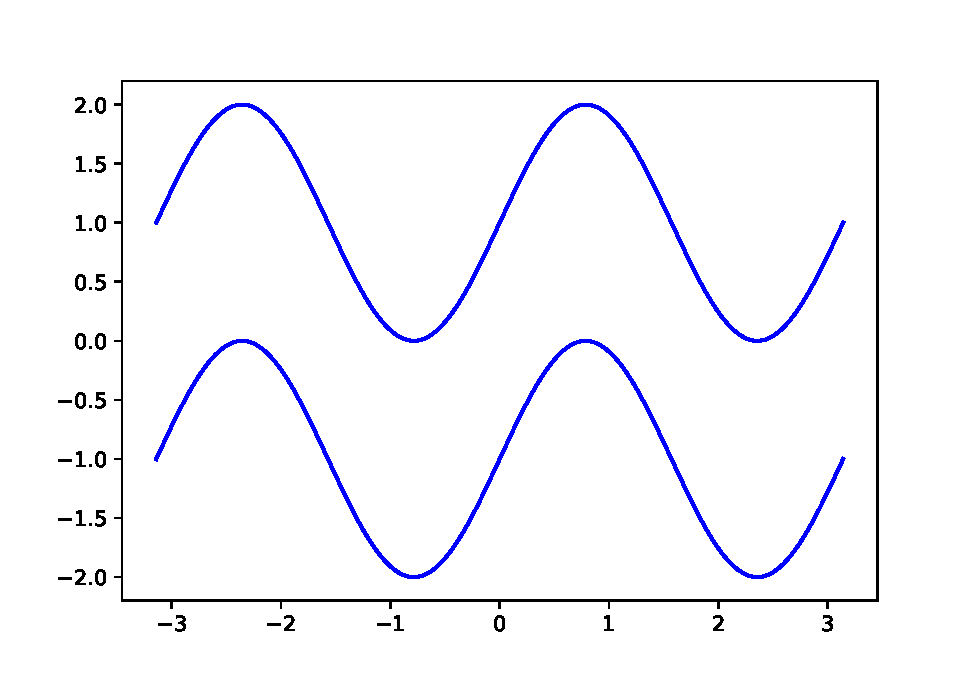
\includegraphics{macd_files/figure-latex/unnamed-chunk-2-1.pdf}

\subsection{EMAN}\label{eman}

\begin{Shaded}
\begin{Highlighting}[]
\KeywordTok{def}\NormalTok{ calculate\_ema(data, window):}
\NormalTok{    alpha }\OperatorTok{=} \DecValTok{2} \OperatorTok{/}\NormalTok{ (window }\OperatorTok{+} \DecValTok{1}\NormalTok{)}
\NormalTok{    ema }\OperatorTok{=}\NormalTok{ data.copy()}
\NormalTok{    ema.iloc[}\DecValTok{0}\NormalTok{] }\OperatorTok{=}\NormalTok{ data.iloc[}\DecValTok{0}\NormalTok{]}

    \ControlFlowTok{for}\NormalTok{ i }\KeywordTok{in} \BuiltInTok{range}\NormalTok{(}\DecValTok{1}\NormalTok{, }\BuiltInTok{len}\NormalTok{(data)):}
\NormalTok{        ema.iloc[i] }\OperatorTok{=}\NormalTok{ alpha }\OperatorTok{*}\NormalTok{ data.iloc[i] }\OperatorTok{+}\NormalTok{ (}\DecValTok{1} \OperatorTok{{-}}\NormalTok{ alpha) }\OperatorTok{*}\NormalTok{ ema.iloc[i }\OperatorTok{{-}} \DecValTok{1}\NormalTok{]}

    \ControlFlowTok{return}\NormalTok{ ema}
\end{Highlighting}
\end{Shaded}


\end{document}
